% !TeX program = xelatex
\documentclass[10pt]{beamer}

\usetheme{metropolis}

\usepackage{pgfplots}
\usepgfplotslibrary{fillbetween}
\usepackage{pgfopts}
\usepackage{amsmath}
\usepackage{structuralanalysis}
\usepackage{tikz}
\usepackage{tikz-3dplot}
\usepackage{chngcntr}
\usepackage{wasysym}
\usepackage{mathtools}
\usepackage{alphalph}
\usepackage{xcolor}
\usepackage[showdow=false, en-US]{datetime2}
\usepackage{hyperref}

\newcommand{\highlight}[1]{%
	\colorbox{red!50}{$\displaystyle#1$}}

\setcounter{lecture}{20}
\counterwithin{equation}{lecture}
\makeatletter
\def\user@resume{resume}
\def\user@intermezzo{intermezzo}
%
\newcounter{previousequation}
\newcounter{lastsubequation}
\newcounter{savedparentequation}
\setcounter{savedparentequation}{1}
% 
\renewenvironment{subequations}[1][]{%
	\def\user@decides{#1}%
	\setcounter{previousequation}{\value{equation}}%
	\ifx\user@decides\user@resume 
	\setcounter{equation}{\value{savedparentequation}}%
	\else  
	\ifx\user@decides\user@intermezzo
	\refstepcounter{equation}%
	\else
	\setcounter{lastsubequation}{0}%
	\refstepcounter{equation}%
	\fi\fi
	\protected@edef\theHparentequation{%
		\@ifundefined {theHequation}\theequation \theHequation}%
	\protected@edef\theparentequation{\theequation}%
	\setcounter{parentequation}{\value{equation}}%
	\ifx\user@decides\user@resume 
	\setcounter{equation}{\value{lastsubequation}}%
	\else
	\setcounter{equation}{0}%
	\fi
	\def\theequation  {\theparentequation  \alph{equation}}%
	\def\theHequation {\theHparentequation \alph{equation}}%
	\ignorespaces
}{%
%  \arabic{equation};\arabic{savedparentequation};\arabic{lastsubequation}
\ifx\user@decides\user@resume
\setcounter{lastsubequation}{\value{equation}}%
\setcounter{equation}{\value{previousequation}}%
\else
\ifx\user@decides\user@intermezzo
\setcounter{equation}{\value{parentequation}}%
\else
\setcounter{lastsubequation}{\value{equation}}%
\setcounter{savedparentequation}{\value{parentequation}}%
\setcounter{equation}{\value{parentequation}}%
\fi\fi
%  \arabic{equation};\arabic{savedparentequation};\arabic{lastsubequation}
\ignorespacesafterend
}
\makeatother
\title{AE 737 - Mechanics of Damage Tolerance}
\subtitle{Lecture \arabic{lecture}}
\date{Last Updated: \today\ at \DTMcurrenttime}
\author{Dr. Nicholas Smith}
\institute{Wichita State University, Department of Aerospace Engineering}
% \titlegraphic{\hfill\includegraphics[height=1.5cm]{logo/logo}}

\begin{document}

\maketitle
\begin{frame}{schedule}
	\begin{itemize}
		\item 7 Apr - Crack Growth, Stress Spectrum
		\item 12 Apr - Retardation, Boeing Commercial Method
		\item 14 Apr - Exam Review, Homework 8 Due
		\item 19 Apr - Damage Tolerance
		\item 21 Apr - Exam 2
		\item 26 Apr - Exam Solutions, Damage Tolerance
%		\item 28 Apr - AFGROW, Finite Elements
%		\item 3 May - Finite Elements
%		\item 5 May - Non-Destructive Testing, Composites, Final Project Due May 10
	\end{itemize}
\end{frame}

\begin{frame}{office hours}
	\begin{itemize}
		\item I have a meeting this Friday afternoon (4/8)
		\item Office hours will be Monday 4/11 from 3:00 - 5:00
		\item As always you can e-mail me to schedule another time, or ask your questions via e-mail
	\end{itemize}
\end{frame}

\begin{frame}
  \frametitle{outline}
  \setbeamertemplate{section in toc}[sections numbered]
  \tableofcontents[hideallsubsections]
\end{frame}

\section{crack growth rate}

\begin{frame}{fracture surface}
	\begin{figure}
	\centering
	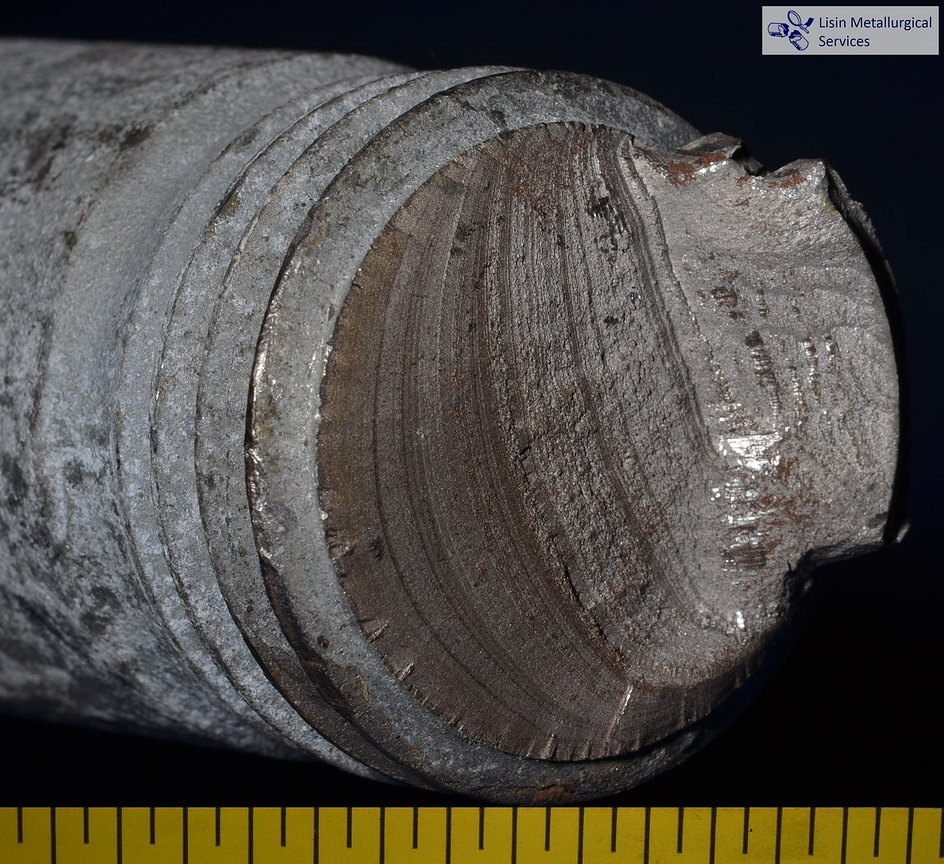
\includegraphics[width=0.7\linewidth]{../Figures/fracture_surface}
	\label{fig:fracture_surface}
	\end{figure}
\end{frame}

\begin{frame}{fracture surface}	
	\begin{figure}
	\centering
	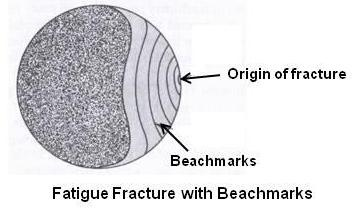
\includegraphics[width=0.7\linewidth]{../Figures/Fatigue-Fracture-with-Beachmarks}
	\label{fig:Fatigue-Fracture-with-Beachmarks}
	\end{figure}
\end{frame}

\begin{frame}{crack growth rate}
	\begin{itemize}[<+->]
		\item Crack growth rate can be measured experimentally 
		\item Using a center-crack specimen, a fatigue load is applied
		\item The crack length is measured and plotted vs. the number of cycles
		\item The slope of this curve ($\frac{da}{dN}$) is then plotted vs. either $K_{I,max}$ or $\Delta K_I$ on a log-log scale
		\item This chart is then commonly divided into three regions
	\end{itemize}
\end{frame}

\begin{frame}{da-dN vs K}	
	\begin{figure}
	\centering
	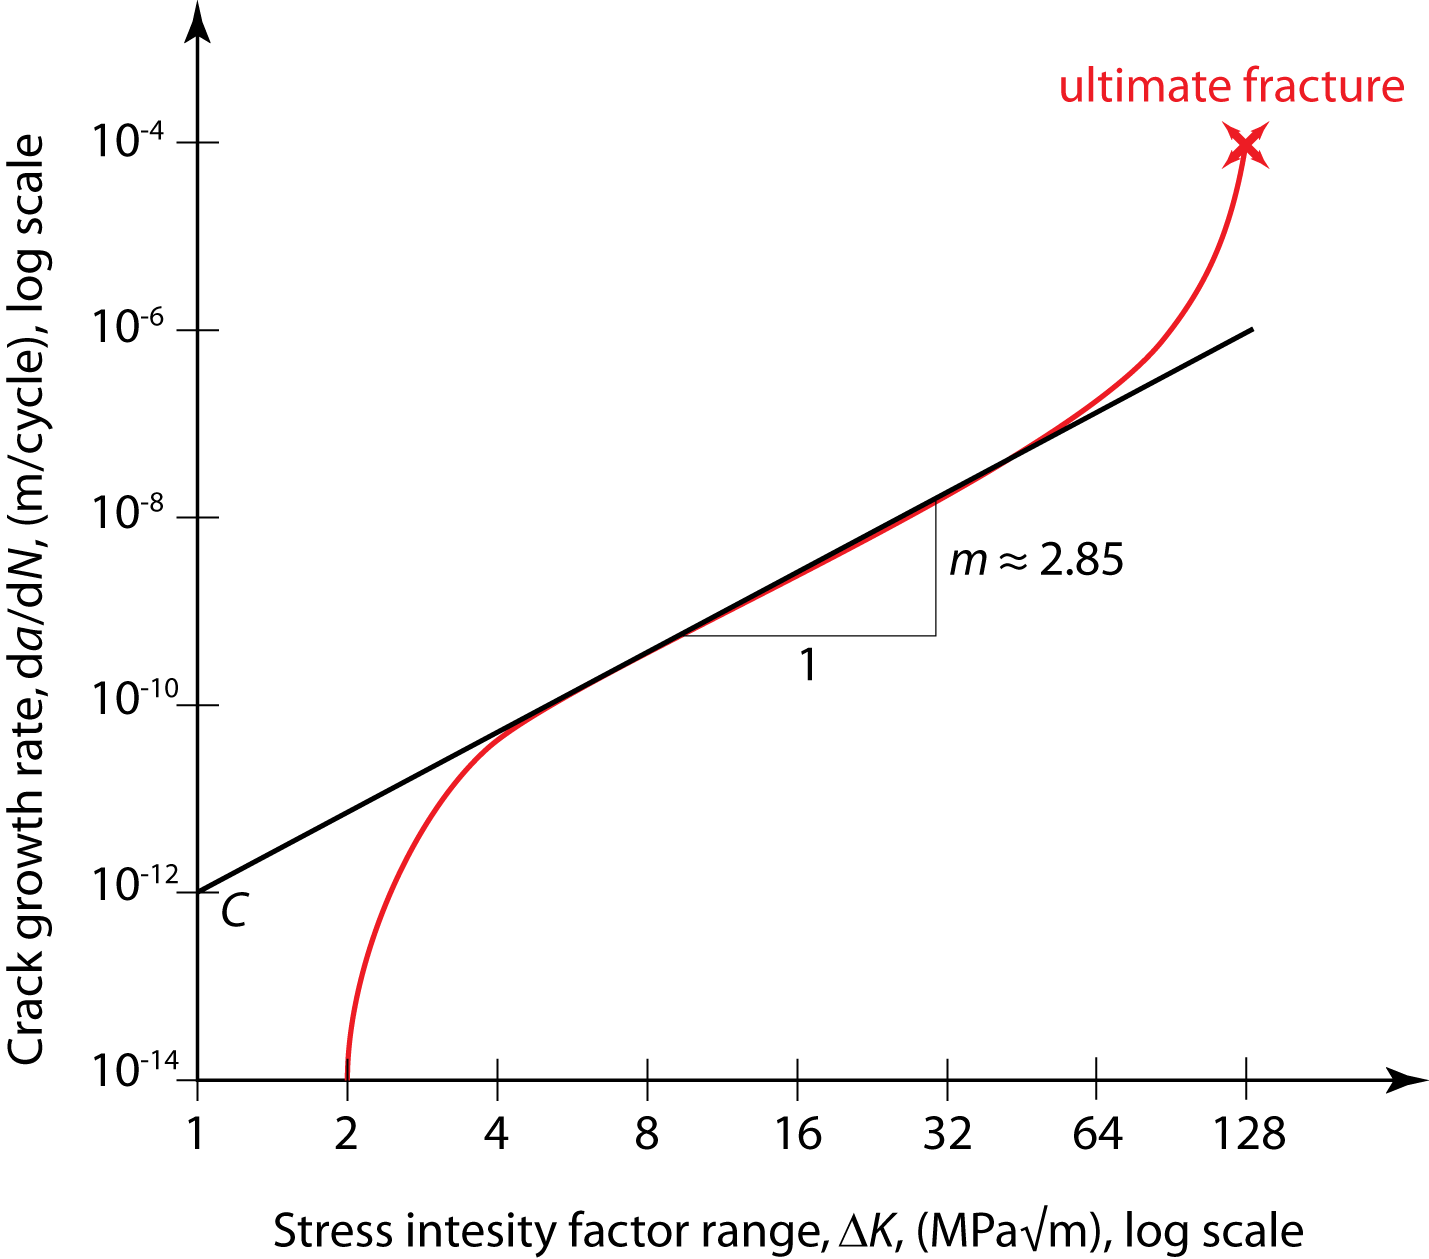
\includegraphics[width=0.7\linewidth]{../Figures/da-dn}
	\label{fig:da-dn}
	\end{figure}
\end{frame}

\begin{frame}{region I}
	\begin{itemize}[<+->]
		\item In Region I crack growth is very slow and/or difficult to measure
		\item In many cases, da/dN corresponds to the spacing between atoms!
		\item The point at which the da/dN curve intersects the x-axis is known as the fatigue threshold, $K^{th}$
		\item Typically 3-15 $\text{ ksi} \sqrt{\text{in}}$ for steel
		\item 3-6 $\text{ ksi} \sqrt{\text{in}}$ for aluminum
	\end{itemize}
\end{frame}

\begin{frame}{region II}
	\begin{itemize}[<+->]
		\item Most important region for general engineering analysis
		\item Once a crack is present, most of the growth and life occurs in Region II
		\item Generally linear in the log-log scale
	\end{itemize}
\end{frame}

\begin{frame}{region III}
	\begin{itemize}[<+->]
		\item Unstable crack growth
		\item Usually neglected (we expect failure before Region III fully develops in actual parts)
		\item Can be significant for parts where we expect high stress and relatively short life
	\end{itemize}
\end{frame}

\begin{frame}{crack growth rate curve}
	\begin{itemize}[<+->]
		\item The crack growth rate curve is considered a material property
		\item The same considerations for thickness apply as with fracture toughness ($K_c$ vs. $K_{Ic}$) 
		\item Is also a function of the load ratio, $R = \sigma_{min}/\sigma_{max}$
	\end{itemize}
\end{frame}

\begin{frame}{R effects}
	\begin{itemize}[<+->]
		\item While the x-axis can be either $\Delta K$ or $K_{max}$, the shape of the data is the same
		\item When we look at the effects of load ratio, $R$, the axis causes some differences on the plot
		\item With $\Delta K$ on the x-axis, increasing $R$ will shift the curve up and to the left, shifting the fatigue threshold and fracture toughness on the graph as well
		\item With $K_{max}$ on the x-axis, increasing $R$ shifts the curve down and to the right, but fatigue threshold and fracture toughness keep same values
		\item In general, $R$ dependence vanishes for $R> 0.8$ or $R<-0.3$. This effect is known as the band width
	\end{itemize}
\end{frame}

%TODO - Paris Law example
\begin{frame}{paris example}
	
\end{frame}

\section{factors affecting crack propagation}

\begin{frame}{factors affecting crack propagation}
	\begin{itemize}[<+->]
		\item thickness
		\item stress ratio
		\item temperature
		\item environment
		\item frequency
		\item crack orientation
		\item manufacturer
		\item heat treatment
	\end{itemize}
\end{frame}

\begin{frame}{thickness}
	\begin{itemize}[<+->]
		\item We already discussed the effects of thickness on fracture toughness
		\item The same effects are important in crack propagation
		\item In thin (plane stress) plates, cracks can be treated as through cracks
		\item In thick plates (plain strain), we generally need to consider the crack shape
	\end{itemize}
\end{frame}

\begin{frame}{thickness}
	\begin{itemize}[<+->]
		\item Cyclic life is primarily a function of $K_i / K_c$ where $K_i$ is the stress intensity factor in the first cycle
		\item Other experiments indicate a relationship between $\frac{d(a/Q)}{dN}$ and $K_{max}$
		\item $Q$ is a shape parameter for elliptical flaws
	\end{itemize}
\end{frame}

\begin{frame}{temperature}
	\begin{itemize}[<+->]
		\item In general (for most aluminum alloys) cracks propagate more slowly with a decrease in temperature
		\item This trend is exactly opposite the trend for $K_c$
		\item The effect varies in different materials
		\item Most materials benefit from slightly lower temperatures, but as temperatures are further decreased the crack growth rate increases again
	\end{itemize}
\end{frame}

\begin{frame}{temperature}
	\begin{figure}
	\centering
	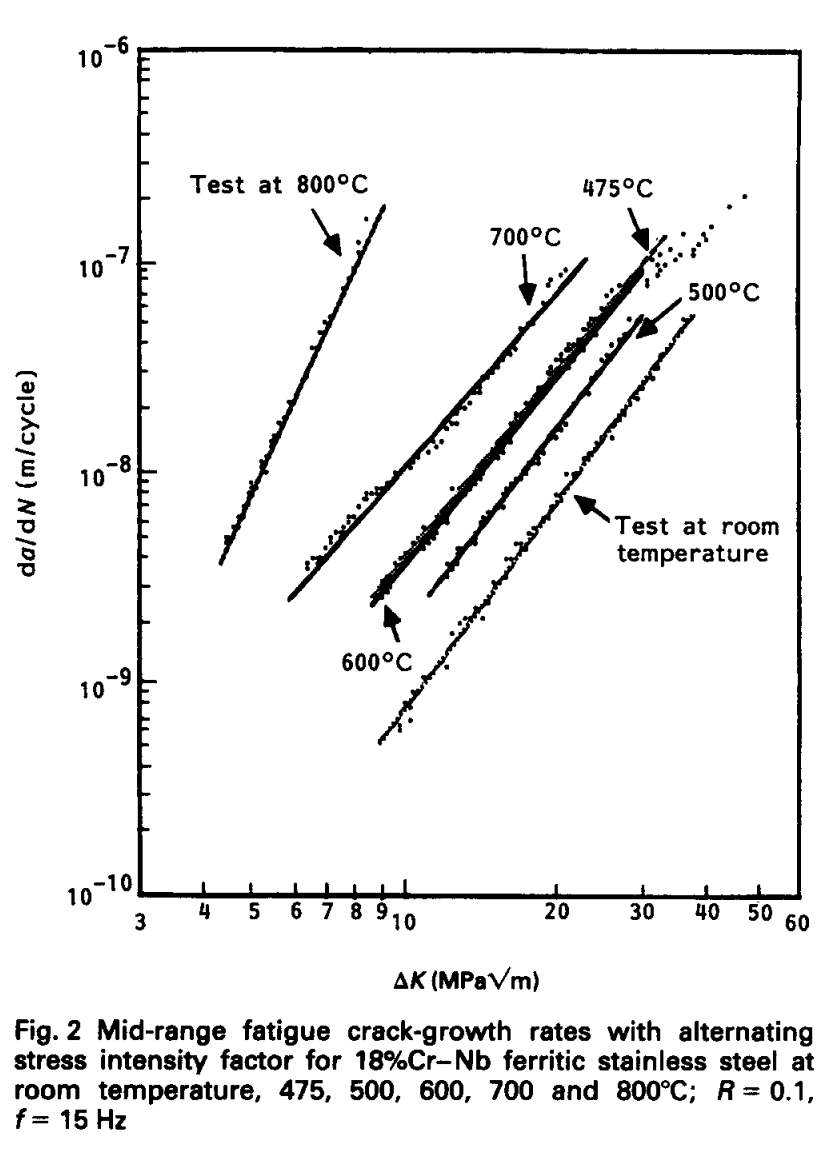
\includegraphics[width=0.6\linewidth]{../Figures/temperature_growth}
	\label{fig:temperature_growth}
	\end{figure}
\end{frame}

\begin{frame}{temperature}
	\begin{itemize}[<+->]
		\item In general, temperature effects can not be predicted well
		\item Instead, materials should be tested at a range of temperatures to establish a range of operating temperatures with corresponding crack growth data
	\end{itemize}
\end{frame}

\begin{frame}{environment}
	\begin{itemize}[<+->]
		\item There are many conditions in the environment that can affect crack growth
		\item Moisture greatly increases the crack growth rate
		\item Salt water increases crack growth rate even further
		\item These effects have varying strength depending on the material used
	\end{itemize}
\end{frame}

\begin{frame}{environment}
	\begin{columns}
		\begin{column}{0.45\textwidth}
			\begin{figure}
			\centering
			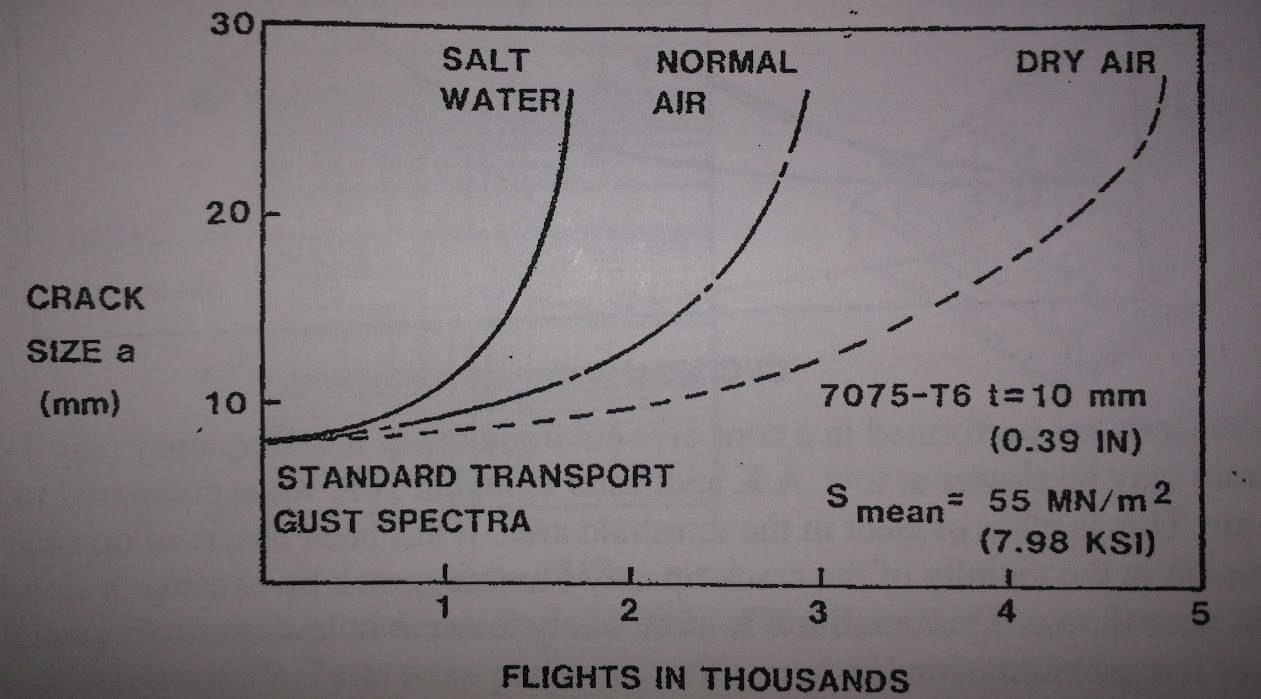
\includegraphics[width=1.0\linewidth]{../Figures/environment_7075}
			\label{fig:environment_7075}
			\end{figure}
		\end{column}
		\begin{column}{0.45\textwidth}
			\begin{figure}
			\centering
			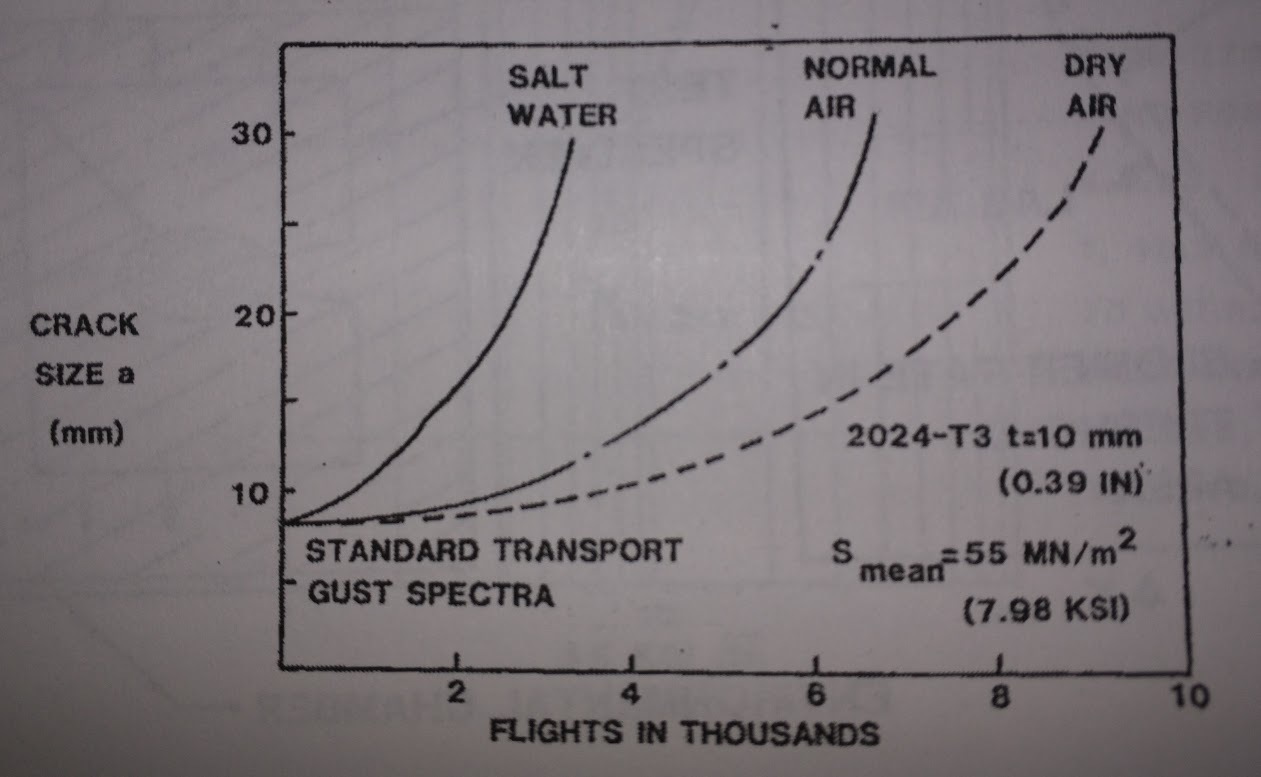
\includegraphics[width=1.0\linewidth]{../Figures/environment_2024}
			\label{fig:environment_2024}
			\end{figure}
		\end{column}
	\end{columns}
\end{frame}

\begin{frame}{environment}
	\begin{itemize}[<+->]
		\item Further, the shape of the applied load curve has a significant effect when combined with adverse environments
		\item Crack growth is faster when the load increases slowly and decreases rapidly
		\item Crack growth is slower when the load increases rapidly and decreases slowly
	\end{itemize}
\end{frame}

\begin{frame}{environment}
	\begin{itemize}[<+->]
		\item When the environment is corrosive, the test frequency is of particular importance
		\item At low frequencies, a corrosive environment increases the threshold, $K^{th}$
		\item However in Region II, crack growth is faster
		\item This effect can be explained by the corrosive environment blunting the crack tip
	\end{itemize}
\end{frame}

\begin{frame}{frequency}
	\begin{itemize}[<+->]
		\item There is conflicting information about the effect of frequency in the absence of a corrosive environment
		\item Some experiments have found a frequency dependence, while others have not
		\item Many claim that the frequency dependence is due to small amounts of water in air during frequency dependence experiment
	\end{itemize}
\end{frame}

\begin{frame}{crack orientation}
	\begin{itemize}[<+->]
		\item For rolled plates, a crack will generally propagate faster parallel to the rolling direction
		\item In many materials, however, the difference between orientations is not significant when compared to scatter, and it is often neglected
		\item Some materials behave very differently with different crack orientations (i.e. the slope of the paris law curve is different), so care should be taken based on the material used
	\end{itemize}
\end{frame}

\begin{frame}{manufacturer}
	\begin{itemize}[<+->]
		\item Different manufacturers of the same material can produce different crack growth rates
		\item Some reasons for this may be
		\item Slight variation in composition
		\item Site cleanliness (inclusions)
		\item Heat treatment/cold rolling variations
	\end{itemize}
\end{frame}

\begin{frame}{heat and surface treatments}
	\begin{itemize}[<+->]
		\item Different heat and surface treatments are often applied
		\item They provide various benefits (corrosion resistance, residual stress, residual stress relief)
		\item But they will also affect the crack growth rate
	\end{itemize}
\end{frame}

\section{numerical algorithm}

\begin{frame}{numerical algorith}
\begin{itemize}[<+->]
	\item While the Paris Law can be integrated directly (for simple load cases), many of the other formulas cannot
	\item A simple numerical algorithm for determining incremental crack growth is
	\item[]	\begin{equation}
	a_{i+1} = a_i + \left(\frac{da}{dN}\right)_i\left(\Delta N\right)_i
	\end{equation}
	\item This method is quite tedious by hand (need many $a_i$ values for this to be accurate) 
	\item But is simple to do in Excel, MATLAB, Python, or many other codes
	\item For most accurate results, use $\Delta N = 1$, but this is often unnecessary
	\item When trying to use large $\Delta N$, check convergence by using larger and smaller $\Delta N$ values
\end{itemize}
\end{frame}

%TODO - Boeing-Walker example
\begin{frame}{boeing-walker example}
	
\end{frame}

%TODO - Convergence example
\begin{frame}{convergence example}
	
\end{frame}

\begin{frame}{variable load cases}
	\begin{itemize}[<+->]
		\item In practice variable loads are often seen
		\item The most basic way to handle these is to simply calculate the crack length after each block of loading
		\item We will discuss an alternate method, which is more convenient for flight "blocks" next class
		\item We will also discuss "retardation" models next class
	\end{itemize}
\end{frame}

%TODO - Variable load example
\begin{frame}{variable load example}
	
\end{frame}

\end{document}
